%%%%%%%%%%%%%%%%%%%%%%%%%%%%%%%%%%%%%%%%%%%%%%%%%%%%%%%%%%%%
%%  This Beamer template was created by Cameron Bracken.
%%  Anyone can freely use or modify it for any purpose
%%  without attribution.
%%
%%  Last Modified: January 9, 2009
%%

\documentclass[xcolor=x11names,compress]{beamer}

%% General document %%%%%%%%%%%%%%%%%%%%%%%%%%%%%%%%%%
\usepackage{graphicx}

\usepackage{xcolor}

\usepackage{pgffor} 

%%%%%%%%%%%%%%%%%%%%%%%%%%%%%%%%%%%%%%%%%%%%%%%%%%%%%%

\usepackage[frenchb]{babel}

\usepackage[utf8]{inputenc}

\usepackage{lastpage}

\usepackage[natbib=true, bibstyle=authoryear,
citestyle=authoryear, backend=biber]{biblatex}

\usepackage{caption}
\captionsetup{figurename=}

\usepackage{appendixnumberbeamer}

\resetcounteronoverlays{lstnumber}

%% Beamer Layout %%%%%%%%%%%%%%%%%%%%%%%%%%%%%%%%%%
\useoutertheme[subsection=false,shadow]{miniframes}
\useinnertheme{default} \usefonttheme{serif} 
\usepackage{palatino}

\setbeamerfont{title like}{shape=\scshape}
\setbeamerfont{title}{shape=\scshape}
\setbeamerfont{frametitle}{shape=\scshape}
\setbeamerfont{footline}{shape=\scshape}

\definecolor{MRed}{HTML}{8B0000} \definecolor{MGreen}{HTML}{008B00}
\definecolor{MBlue}{HTML}{00688B}

\setbeamercolor*{lower separation line head}{bg=MBlue}
\setbeamercolor*{normal text}{fg=black,bg=white}
\setbeamercolor*{alerted text}{fg=red} \setbeamercolor*{example
  text}{fg=black} \setbeamercolor*{structure}{fg=black}

\setbeamercolor*{palette tertiary}{fg=black,bg=black!10}
\setbeamercolor*{palette quaternary}{fg=black,bg=black!10}

\setbeamercolor{footlinerule}{bg=MBlue}
\setbeamercolor*{footlinecolor}{bg=black!10}

\setbeamercolor{block title}{use=structure,fg=white,bg=MBlue!75!black}
\setbeamercolor{block body}{use=structure,fg=black,bg=MBlue!20!white}

\setbeamercolor{block title
  example}{use=structure,fg=white,bg=MGreen!75!black}
\setbeamercolor{block body
  example}{use=structure,fg=black,bg=MGreen!20!white}

\setbeamercolor{block title
  alerted}{use=structure,fg=white,bg=MRed!75!black}
\setbeamercolor{block body
  alerted}{use=structure,fg=black,bg=MRed!20!white}

\renewcommand{\(}{\begin{columns}} \renewcommand{\)}{\end{columns}}
\newcommand{\<}[1]{\begin{column}{#1}} \renewcommand{\>}{\end{column}}
%%%%%%%%%%%%%%%%%%%%%%%%%%%%%%%%%%%%%%%%%%%%%%%%%%


\author{Arnaud Bletterer} \title{Outils multidimensionnels de
  déformation}

\newcommand{\mytext}{Outils multidimensionnels de déformation}

\graphicspath{{PresentationFigs/}}

%%%%%%%%%%%%%%%%%%%%%%%%%%%%%%%%%%%%%%%%%%%%%%%%%%%%%%
%%%%%%%%%%%%%%%%%%%%%%%%%%%%%%%%%%%%%%%%%%%%%%%%%%%%%%

\makeatother \setbeamertemplate{footline} {%
  \leavevmode
  \begin{beamercolorbox}[wd=\paperwidth,ht=1ex,dp=0ex,center]{footlinerule}
  \end{beamercolorbox}%



  \hbox{\begin{beamercolorbox}[wd=1\paperwidth,ht=2.5ex,dp=1.125ex,leftskip=.3cm,rightskip=.3cm]{footlinecolor}%
      \count1 = \linewidth \divide\count1 by \inserttotalframenumber

      \foreach \n in {1,...,\insertframenumber}{\hskip1.\count1}
      
\includegraphics[scale=0.06, viewport= 400 200 0 0]{cgogn}
   
  \end{beamercolorbox}
}

\hbox{\begin{beamercolorbox}[wd=.5\paperwidth,ht=2.5ex,dp=1.125ex,leftskip=.3cm,rightskip=.3cm]{footlinecolor}%
    \inserttitle
  \end{beamercolorbox}%

    \begin{beamercolorbox}[wd=.5\paperwidth,ht=2.5ex,dp=1.125ex,leftskip=.3cm,rightskip=.3cm]{footlinecolor}%
      \usebeamerfont{author in head/foot}\insertauthor\hfill
      \insertframenumber /\inserttotalframenumber
    \end{beamercolorbox}}%
  \vskip0pt%
} \makeatletter

%%%%%%%%%%%%%%%%%%%%%%%%%%%%%%%%%%%%%%%%%%%%%%%%%%%%%%
%%%%%%%%%%%%%%%%%%%%%%%%%%%%%%%%%%%%%%%%%%%%%%%%%%%%%%

\newcommand{\highlightR}[1]{%
  \colorbox{MRed!50}{$\displaystyle#1$}} \newcommand{\highlightB}[1]{%
  \colorbox{MBlue!50}{$\displaystyle#1$}}
\newcommand{\highlightG}[1]{%
  \colorbox{MGreen!50}{$\displaystyle#1$}}
\newcommand{\highlightO}[1]{%
  \colorbox{orange!50}{$\displaystyle#1$}}
\newcommand{\highlightV}[1]{%
  \colorbox{violet!50}{$\displaystyle#1$}}
\newcommand{\highlightGR}[1]{%
  \colorbox{gray!50}{$\displaystyle#1$}}


%%%%%%%%%%%%%%%%%%%%%%%%%%%%%%%%%%%%%%%%%%%%%%%%%%%%%%
%%%%%%%%%%%%%%%%%%%%%%%%%%%%%%%%%%%%%%%%%%%%%%%%%%%%%%

\bibliography{../Rapport/References/references.bib}
\begin{document}

%%%%%%%%%%%%%%%%%%%%%%%%%%%%%%%%%%%%%%%%%%%%%%%%%%%%%%
%%%%%%%%%%%%%%%%%%%%%%%%%%%%%%%%%%%%%%%%%%%%%%%%%%%%%%
\begin{frame}
  \title{Outils multidimensionnels de déformation\\~\\

    \begin{figure}
      \begin{center}
        
\includegraphics[scale=0.3]{uds-logo}~~~~~~~~~
        
\includegraphics[scale=0.15]{icube-logo}
      \end{center}
    \end{figure}
  } \author{Arnaud Bletterer \\ \textit{Université de Strasbourg}
    \vspace{-0.5cm} \date{\today} } \titlepage
\end{frame}

%%%%%%%%%%%%%%%%%%%%%%%%%%%%%%%%%%%%%%%%%%%%%%%%%%%%%%
%%%%%%%%%%%%%%%%%%%%%%%%%%%%%%%%%%%%%%%%%%%%%%%%%%%%%%

\begin{frame}{Outils de déformation}
\begin{columns}[t]
  \begin{column}{0.5\textwidth}
    
\includegraphics[scale=0.16]{Outil-Mono-Sans}
  \end{column}
  \pause
  \begin{column}{0.5\textwidth}
    
\includegraphics[scale=0.16]{Outil-Mono-Points}
  \end{column}
  \pause
\end{columns} 
\begin{columns}[t]
  \begin{column}{0.5\textwidth}
    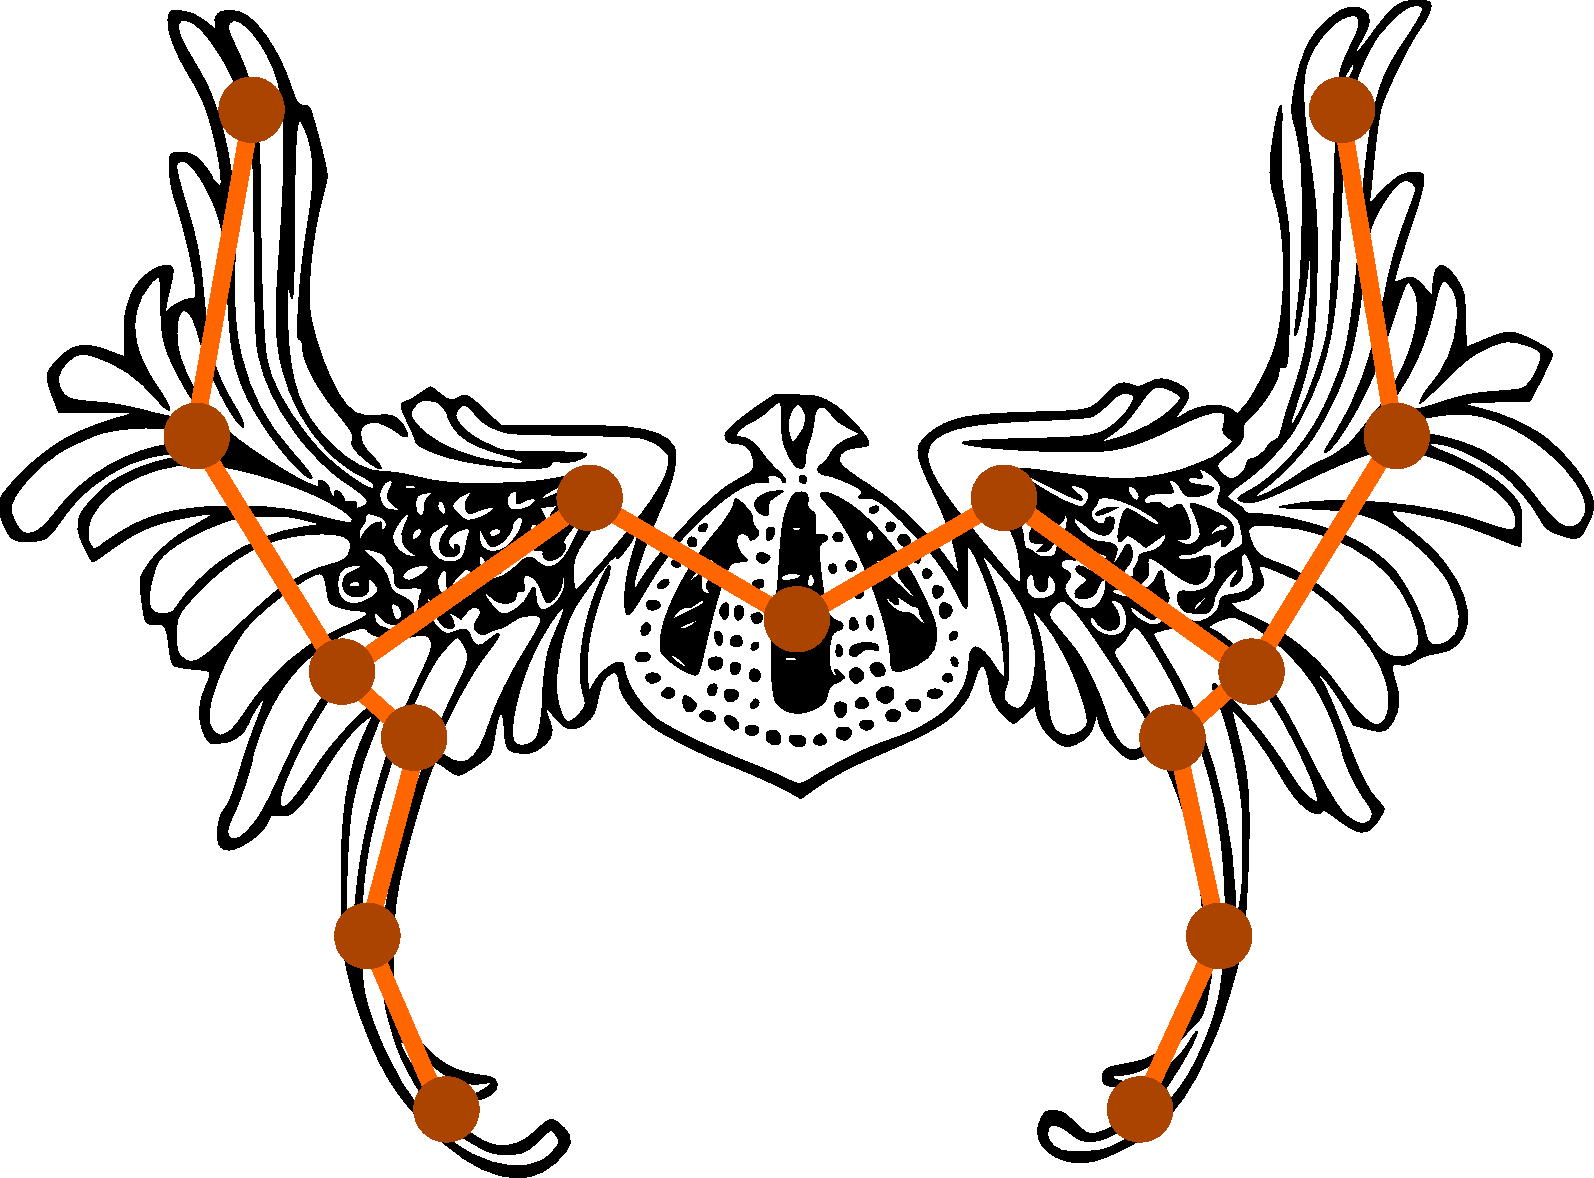
\includegraphics[scale=0.16]{Outil-Mono-Courbes}
  \end{column}
  \pause
  \begin{column}{0.5\textwidth}
    
\includegraphics[scale=0.16]{Outil-Mono-Surfaces}
  \end{column}
\end{columns} 
\end{frame}

\begin{frame}{Problématique}
  \centering
\begin{columns}[t]
  \begin{column}{0.5\textwidth}
    
\includegraphics[scale=0.2]{Outil-Mono-Sans}
  \end{column}
  \pauses
  \begin{column}{0.5\textwidth}
    
\includegraphics[scale=0.2]{Outil-Multi}
  \end{column}
\end{columns} 
\end{frame}

%%%%%%%%%%%%%%%%%%%%%%%%%%%%%%%%%%%%%%%%%%%%%%%%%%%%%%
%%%%%%%%%%%%%%%%%%%%%%%%%%%%%%%%%%%%%%%%%%%%%%%%%%%%%%

\begin{frame}{}
\begin{center}
\huge Merci de votre attention.
\end{center}
\end{frame}

\appendix

\end{document}